\documentclass[../main.tex]{subfiles}

\graphicspath{{../images/}}

\begin{document}
\pagestyle{fancy}
\chead{Module 3}
\rhead{Junseo Shin}
\lhead{CSE 4059}


\renewcommand{\thefigure}{\arabic{figure}}
\section*{Image Color to Grayscale}

\begin{figure}
    [ht]
    \centering
    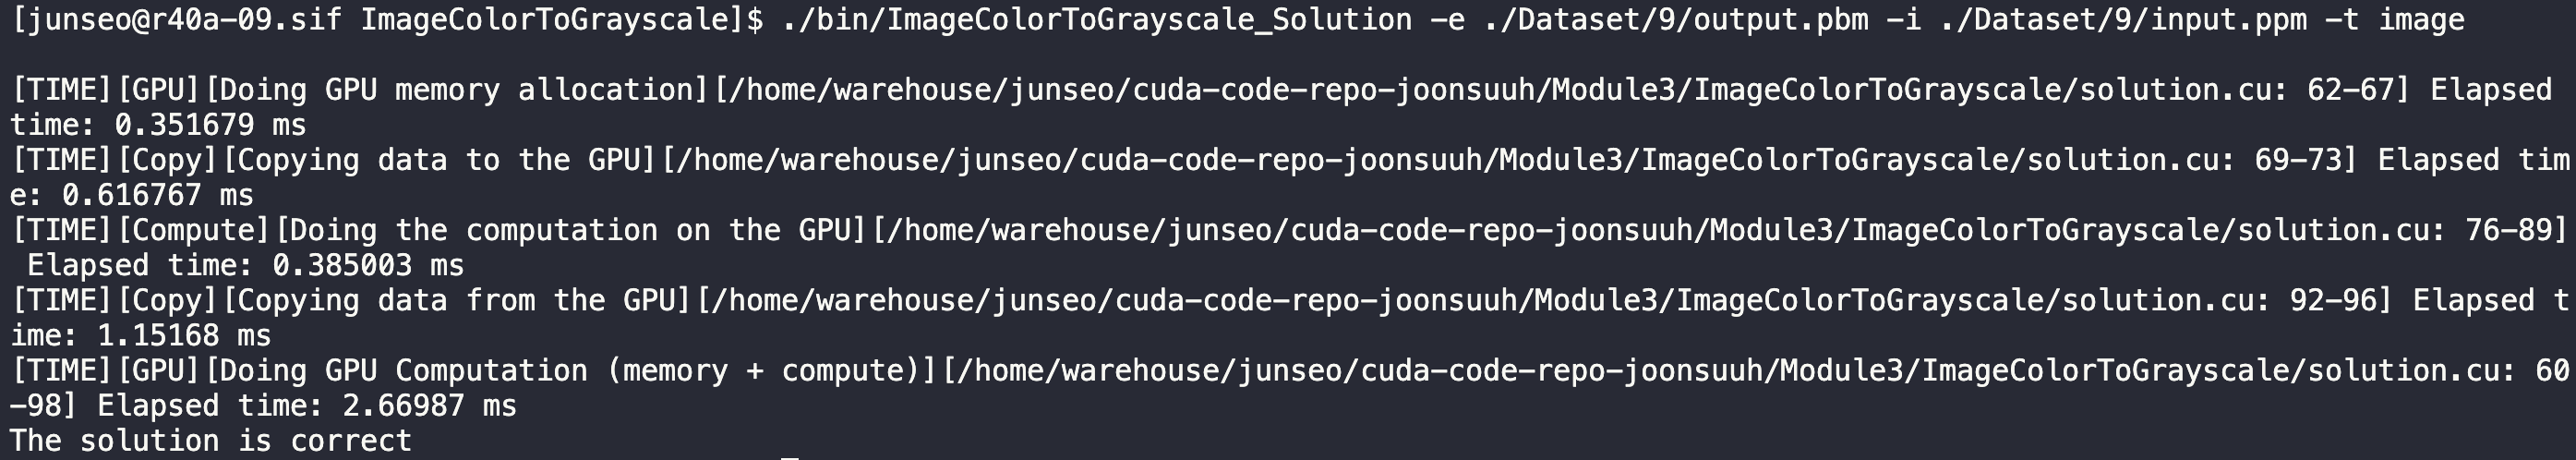
\includegraphics[width=0.8\textwidth]{imagecolortograyscale.png}
    \caption{\texttt{ImageColorToGrayscale\_Solution} output}
\end{figure}

\subsection*{Questions}

\begin{enumerate}
    \item How many floating-point operations are being performed in your color
    conversion kernel? EXPLAIN.

    The kernel performs \texttt{imageWidth * imageHeight * 5} floating-point operations.
    Each thread (\texttt{imageWidth * imageHeight}) in the if statement performs
    3 multiplications and 2 additions.

    \item Which format would be more efficient for color conversion: a 2D matrix
    where each entry is an RGB value, or a 3D matrix where each slice in
    the Z axis representes a color? In other words, is it better to have color
    interleaved in this application? Can you name an application where the
    oposite is true?

    It would be more efficient to have a 2D matrix since the threads in the kernel
    would be able to access the RGB values in a single memory read operation.

    An application where it would be better to have color interleaved would be
    an algorithm that uses individual color channels separately---e.g. JPEG compression performs 
    a discrete cosine transform on each converted color channel Y, Cb, Cr separately
    (source \href{https://en.wikipedia.org/wiki/JPEG#JPEG_codec_example}{Wikipedia}).

    \item How many global memory reads are being performed by your kernel?
    EXPLAIN.

    The kernel performs \texttt{imageWidth * imageHeight * 3} global memory reads because
    each thread has to read the three color channels (RGB) from the input image.

    \item How many global memory writes are being performed by your kernel?
    EXPLAIN.

    The kernel performs \texttt{imageWidth * imageHeight} global memory writes because
    each thread writes to the output image in the if statement.

    \item Describe what possible optimizations can be implemented to your kernel
    to achieve a performance speedup.

    Again, we can increase performance with shared memory and using block sizes that are
    a multiple of the warp size (32).

    \item Name three applications for color conversion
    
    \begin{enumerate}
        \item [i] Device compatibility and cameras (all screens and cameras may use different
            color spaces and color channels)
        \item [ii] Printers (printing a color image into grayscale)
        \item [iii] Edge detection; Canny Edge Detection has to first convert the image to grayscale
            before applying the edge detection algorithm!
    \end{enumerate}
\end{enumerate}



\end{document}